\documentclass[../main.tex]{subfiles}
\graphicspath{{\subfix{../images/}}}

\begin{document}


\section{Forecast verification}
\label{sec:fcast_verif}
When evaluating the forecasts produced by the cGAN, there are many different factors we need to assess. First of all we are interested in how realistic the forecasts are, in terms of the spatial distribution, timing and intensity of the rainfall. To assess this we use the Radially Averaged Power Spectral Density (discussed below), quantile-quantile plots, histograms and plots of the diurnal cycle. Second, we are interested in whether the forecast is able to skilfully predict the occurrence of particular events, in this case rainfall exceeding a threshold. To assess this, we use the Equitable Threat Score, and the Fractions Skill Score (discussed below). Lastly we are interested in how well the probability distribution of the GAN ensemble aligns with the distribution of the observed values, for which we use a Spread Error plot and Rank Histogram (discussed below).

One complicating factor in this work is that we produce an ensemble of predictions with the cGAN, but only have deterministic forecasts from the IFS to compare with. We expect the IFS HRES to be similar to a single member of an ensemble, so that we can fairly compare single members of the cGAN ensemble with the IFS forecast. However, we do not have a benchmark ensemble forecast to compare with, and so it is hard to properly assess the quality of the ensemble as a whole.


\subsection{Radially Averaged Power Spectral Density (RAPSD)}
\label{metrics:rapsd}

In order to assess the spatial realism of the generated forecasts, we use the Radially Averaged Power Spectral Density (RAPSD)~\citep{sinclair_empirical_2005, harris_multiscale_2001}. This is calculated by taking the 2D Fourier transform of the precipitation image, and averaging this around the centre of the image, yielding a one-dimensional series showing the distribution of weights given to different frequencies. For assessing multiple forecast images we take the mean RAPSD over the images, and for situations where we need to summarise the overall similarity of two RAPSD curves we use the Radially Averaged Log Spectral Distance (RALSD) defined in~\cite{harris_generative_2022}.

\subsection{Continuous Ranked Probability Score}

The Continuous Ranked Probability Score, or CRPS, is a particularly important score in assessing probabilistic forecasts, as it is a \emph{strictly proper} score~\citep{wilks_statistical_2019}, in that the score is only maximised when the forecast distribution equals the target distribution. For a cumulative forecast distribution $F(y)$, the CRPS for an observed occurrence of $x$ (e.g. observed rainfall value) is defined as:
\begin{align}
    \text{CRPS}(F, x)= \int_{-\infty}^{\infty} \left[ F(y) - \mathbf{1}_{y\geq x} \right]^2
dy\end{align}
where $\mathbf{1}_{y\geq x}$ is the Heaviside step function. The CRPS is a univariate measure, so does not properly account for spatial correlations. Whilst there is a multivariate generalisation of the CRPS, the energy score~\citep{gneiting_strictly_2007}, the CRPS is more commonly used and has been used in previous related works, so we use it in this work as one of many validation metrics, in order to choose the best model. 





\subsection{Equitable Threat Score and Critical Success Index}
\label{metrics:ets}
In order to assess how well a forecast does at predicting where and when specific events will occur (e.g.~rainfall over 5mm/hr), a commonly used technique is to create a contingency table; for precipitation we divide the rainfall into bins, and create a table showing the relationship between the forecast categories and the observed categories. In this work, we only consider yes/no events such that the contingency table is particularly simple and takes the form in Table~\ref{tab:contingency}.
\begin{table}[]
    \centering
    \begin{tabular}{c|c c}
    & Observation Negative & Observation Positive\\
    \hline
      Forecast Negative & True Negative (TN) &  False Negative (FN) \\
      Forecast Positive & False Positive (FP) &  True Positive (TP)
    \end{tabular}
    \caption{The structure of a contingency table for an event with two outcomes (e.g. rain / no rain).}
    \label{tab:contingency}
\end{table}

Rather than comparing many of these tables, it is easier to summarise this table using a summary score~\citep{wilks_forecast_2019}, although any score we choose will always imperfectly represent the forecast performance, and so we must be careful with which summary metric we use. The most obvious summary metrics are the Hit Rate (HR, also known as recall or probability of detection) and False Alarm Rate (FAR), defined as:
\begin{align}
    \text{HR} := \frac{\text{TP}}{\text{TP} + \text{FN}}\\
    \text{FAR}:= \frac{\text{FP}}{\text{TP} + \text{FP}}
\end{align}
where TP, TN, FP, FN are the number of true positives, true negatives, false positives and false negatives respectively (see Table~\ref{tab:contingency}). These metrics are useful, but not when evaluated in isolation, since it is easy to artificially achieve perfect scores on either metric (e.g.~we can achieve HR=1 by forecasting that the event will happen every time).

A metric that measures the balance of HR and FAR together is the Critical Success Index (CSI), also known as the Threat Score~\citep{wilks_forecast_2019}; this takes the form
\begin{align}
\text{CSI} := \frac{\text{TP}}{\text{TP} + \text{FP} + \text{FN}}
\end{align}
 The CSI only concerns events for which either the forecast predicted the event to occur, or where the event did occur. The CSI can be rewritten as~\citep{schaefer_critical_1990}:
\begin{align}
    \text{CSI} &= \left[ \frac{1}{\text{POD}} + \frac{1}{1-\text{FAR}} - 1\right] =\left[ \frac{2}{H(\text{POD},{1-\text{FAR}})} - 1\right]
\end{align}
where $H(x,y)$ is the harmonic mean of $x$ and $y$. Thus the CSI depends on the joint values of the HR and FAR and so should enable us to pick models that achieve a balance of HR and FAR.

However, in~\cite{schaefer_critical_1990} it is demonstrated that the CSI is also sensitive to the frequency of the event occurring, and so it is a biased score. In order to remove this bias, a related score, known as the equitable threat score (ETS) or Gilberts Skill Score, can be constructed~\citep{schaefer_critical_1990, wilks_forecast_2019}. This has a similar form to the CSI except that the probability of random events occurring is taken into account:
\begin{align}
\label{eq:ets}
\text{ETS} := \frac{\text{TP} - \text{TP}_{r}}{\text{TP} + \text{FP} + \text{FN} - \text{TP}_{r}}
\end{align}
where $\text{TP}_{r}$ accounts for the number of true positives we would expect to achieve by guessing at random. $\text{TP}_{r}$ can be estimated from climatology, or else estimated from the data by:
\begin{align}
    \text{TP}_{r} = \frac{(\text{TP} + \text{FP})(\text{TP} + \text{FN})}{N}
\end{align}
where $N$ is the total number of observed events (including True Negative events). The ETS is used in operational forecast verification~\citep{mittermaier_long-term_2013} and in~\cite{manzato_behaviour_2017} was shown to be one of the most robust metrics with respect to random (unskillful) changes in the forecast.

\subsection{Fractions Skill Score}
\label{metrics:fss}


\begin{figure}[h]
     \centering
     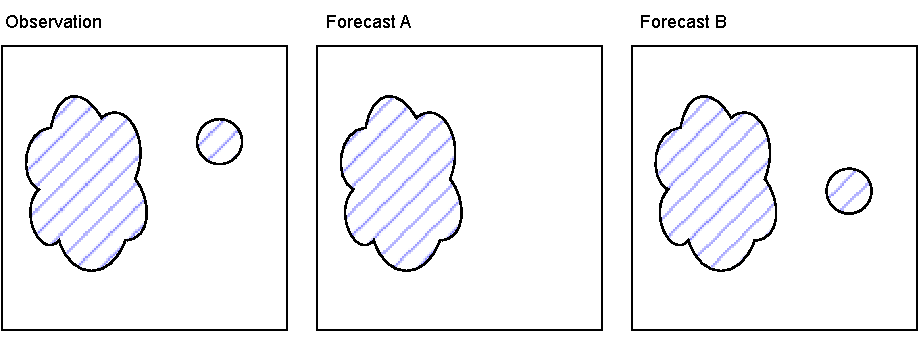
\includegraphics[width=0.85\textwidth]{images/double_penalty.pdf}
     
     \caption{A toy example of observations and two forecasts.}
     \label{fig:double_penalty}
\end{figure}

Many forecast verification scores, such as mean square error or the ETS don't always align with the intuition that a human forecaster has when they evaluate a forecast by eye. As a toy example, consider two forecasts A and B, and corresponding observations shown in Fig.~\ref{fig:double_penalty}. A and B predict the same rainfall pattern in the Western part of the domain, however forecast A incorrectly predicts no rainfall in the East, whereas forecast B correctly predicts the rainfall, but shifted upwards by several grid cells.

If we evaluate these forecasts using the CSI, then forecast B will be penalised twice; once by the presence of False Positives, and once by an increase in False Negatives. Forecast A however is only penalised by an increase in False Negatives. Therefor the CSI will give a higher score to forecast A. 

For the case of the ETS, it isn't immediately obvious which would score higher. Let the smaller precipitation object cover $n$ grid cells, and let $N$ equal the number of grid cells over the whole domain. Then we can write the modifications to the terms in Eq. (\ref{eq:ets}) for forecast B relative to forecast A: 
\begin{align}
    \text{FP}_B &= \text{FP}_A + n \\
    \text{TP}_{r,B} &= \frac{(\text{TP}_A + \text{FP}_A + n)(\text{TP}_A + \text{FN}_A)}{N} = \text{TP}_{r,A} + \frac{n(\text{TP}_A + \text{FN}_A)}{N}
\end{align}
with all other terms remaining equal. Inserting these into Eq. (\ref{eq:ets}) gives:
\begin{align}
\text{ETS}_A &= \frac{\text{TP} -  \text{TP}_{r,A}}{\text{TP} + \text{FP}_A + \text{FN} - \text{TP}_{r,A}} \\
\text{ETS}_B &= \frac{\text{TP} -  \text{TP}_{r,A} - \frac{n}{N}(\text{TP}_A + \text{FN}_A)}{\text{TP} + \text{FP}_A + \text{FN} - \text{TP}_{r,A} + n - \frac{n}{N}(\text{TP}_A + \text{FN}_A)}
\end{align}
Since $\text{TP}_A + \text{FN}_A \leq N$, then $\text{ETS}_B \leq \text{ETS}_A$, and according to the ETS, forecast A is superior. However, many forecasters would prefer forecast B, as it at least captures the correct pattern of rainfall, and often it is not important that the rainfall prediction is in precisely the right place, but that it falls within the right neighbourhood (as we may only be interested in the rainfall over a particular area). 

There have been many different approaches employed to try and remedy this problem (see e.g.~\cite{gilleland_intercomparison_2009}). One way to get around this would be to group the grid cells into particular areas (e.g.~river basins) that we are interested in knowing the rainfall into, and evaluating the forecasts using these groupings. An alternative approach, usually called the neighbourhood approach, is to smooth the forecasts and observations by averaging the forecast around each grid cell with a particular length scale before applying a forecast metric~\citep{ebert_fuzzy_2008, schwartz_comparison_2017, stein_neighborhood-based_2019}. Whilst neighbourhood versions of the ETS have been proposed~\citep{schwartz_comparison_2017}, they are less commonly used as a metric and so we will focus on a more well-used neighbourhood metric, the Fractions Skill Score (FSS)~\citep{roberts_assessing_2008, roberts_scale-selective_2008}.

To calculate the FSS, we first choose a threshold rainfall value $r$, and for each grid cell of the forecast and observations we calculate the fractions $F_{tij}$ and $O_{tij}$ of neighbouring cells for which the rainfall exceeds the threshold, where $t,i$ and $j$ index the time, latitude and longitude axes respectively. The FSS is then defined as:
\begin{align}
    \text{FSS}(n, r) := \frac{\sum_{t=1}^{T}\sum_{i=1}^{N_x} \sum_{j=1}^{N_y} 2 F_{tij}O_{tij}}{\sum_{t=1}^{T}\sum_{i=1}^{N_x}\sum_{j=1}^{N_y} F_{tij}^2 + O_{tij}^2 } \label{eq:fss_main}
\end{align}
The standard approach uses a square neighbourhood, and is typically taken to be along the spatial axes only, but alternative implementations have been suggested that calculate fractions along the time axis~\citep{woodhams_what_2018} and over ensemble members~\citep{duc_spatial-temporal_2013}. We use the pySTEPS implementation of the FSS~\citep{pulkkinen_pysteps_2019}, which performs the averaging using square convolutions with zero-padding

The FSS is typically evaluated relative to the `useful' criteria defined in~\cite{roberts_assessing_2008, roberts_scale-selective_2008}, such that a the neighbourhood length is increased until the score exceeds $\frac{1}{2} + \frac{f_O}{2}$, where $f_O$ is the fraction of pixels exceeding the threshold over the whole observational set. The length scale at which this occurs is typically regarded as the length scale at which the forecast is skilful enough to be used. However, it is known that there can be significant skill for forecasts that do not exceed this threshold~\citep{nachamkin_applying_2015, mittermaier_long-term_2013}. 

Also note that, in the limit of large neighbourhood size, the FSS approaches the asymptotic limit $\text{FSS}_{\infty}$ where~\citep{roberts_scale-selective_2008}:
\begin{align}
\text{FSS}_{\infty} = \frac{2 f_Of_M}{ f_O^2 + f_M^2}
\end{align}
where $f_M$ is the modelled frequency of exceeding the threshold. Thus the value that the FSS reaches at large neighbourhood sizes indicates the level of bias the average number of pixels exceeding the threshold, with $\text{FSS}_{\infty}=1$ for no bias.

\subsection{Spread error}

In order to assess how well calibrated the probabilities of the generated forecast are, we use a spread-error plot, commonly used to assess ensemble calibration~\citep{leutbecher_ensemble_2008}. For an ensemble of forecasts $\{f_{i,t}\}_{i=1}^M$ with ensemble mean $\mu_t$, and an observation $y_t$, the spread $s_t$ and error $e_t$ are defined as:
\begin{align}
    s_t^2 &= \frac{1}{M} \sum_{i=1}^{M} \left( f_{i,t} - \mu_t \right)^2 \\
    e_t^2 &= ( y_t - \mu_t )^2
\end{align}

To produce a spread-error plot, we first calculate the spread values for each grid cell. Then we split the paired observations and forecasts into bins (100 in our case) according to this spread value, and for each bin we calculate the root mean squared spread and error values. Note that for a small number of ensemble members $M$, we need to include a correction term to achieve a corrected spread:
\begin{align}
    \tilde{s}_t = \frac{M+1}{M-1} s_t
\end{align}

\subsection{Rank histogram}
\label{rank_hist}
Another method to assess the statistical calibration of an ensemble forecast is the use of a rank histogram (also known as a Talagrand diagram)~\citep{wilks_forecast_2019}. Consider a sample of $n$ univariate data points, each with an ensemble of $m$ forecasts. To construct a rank histogram, for each sample we rank the observed value relative to the ensemble members, and then average this over all the samples. This gives a frequency of how many times the observations were seen to be in each rank, which can be plotted as a histogram. If the observations behave as if they are drawn from the same distribution as the ensemble members, which is how we would ideally like them to behave, then the observations are equally likely to be in any rank, so that the histogram is flat. For an imperfect ensemble, the spread of the ensemble members may be too wide, such that the observations will rank in the middle most of the time, producing a peak in the histogram. For the reverse scenario, the spread is too narrow leading to a U-shaped histogram indicating too narrow a spread of ensemble members. A histogram sloping to the left or right is also indicative of conditional under-forecasting or over-forecasting respectively~\citep{hamill_interpretation_2001, wilks_forecast_2019}. In this work we use the pySTEPS implementation of the rank histogram~\citep{pulkkinen_pysteps_2019}.

\ifSubfilesClassLoaded{%
    \bibliographystyle{alpha}
    \bibliography{references_z}

}{}


\end{document}